%%%%%%%%%%%%%%%%%%%%%%%%%%%%%%%%%%%%%%%%%
% Journal Article
% LaTeX Template
% Version 2.0 (February 7, 2023)
%
% This template originates from:
% https://www.LaTeXTemplates.com
%
% Author:
% Vel (vel@latextemplates.com)
%
% License:
% CC BY-NC-SA 4.0 (https://creativecommons.org/licenses/by-nc-sa/4.0/)
%
% NOTE: The bibliography needs to be compiled using the biber engine.
%
%%%%%%%%%%%%%%%%%%%%%%%%%%%%%%%%%%%%%%%%%

%----------------------------------------------------------------------------------------
%	PACKAGES AND OTHER DOCUMENT CONFIGURATIONS
%----------------------------------------------------------------------------------------

\documentclass[
	letterpaper, % Paper size, use either a4paper or letterpaper
	10pt, % Default font size, can also use 11pt or 12pt, although this is not recommended
	unnumberedsections, % Comment to enable section numbering
	twoside, % Two side traditional mode where headers and footers change between odd and even pages, comment this option to make them fixed
]{LTJournalArticle}

\addbibresource{bibliography.bib} % BibLaTeX bibliography file

\runninghead{UNC-2452 SolarWinds} % A shortened article title to appear in the running head, leave this command empty for no running head

\footertext{\textit{Report2} (MICS CYBER 204, Summer-2024)} % Text to appear in the footer, leave this command empty for no footer text

\setcounter{page}{1} % The page number of the first page, set this to a higher number if the article is to be part of an issue or larger work

%----------------------------------------------------------------------------------------
%	TITLE SECTION
%----------------------------------------------------------------------------------------

\usepackage[title,toc,titletoc]{appendix}
\usepackage{titlesec}
\usepackage{lscape}


\title{SolarWinds \\ MICS-204 Report 2, Summer 2024} % Article title, use manual lines breaks (\\) to beautify the layout

% Authors are listed in a comma-separated list with superscript numbers indicating affiliations
% \thanks{} is used for any text that should be placed in a footnote on the first page, such as the corresponding author's email, journal acceptance dates, a copyright/license notice, keywords, etc
\author{
	Karl-Johan Westhoff \\
	email \href{mailto:kjwesthoff@berkeley.edu}{kjwesthoff@berkeley.edu}
}

% Affiliations are output in the \date{} command
\date{UC Berkleley School of Information \\
MICS Course 204 Summer 2024
}

% % Full-width abstract
% \renewcommand{\maketitlehookd}{%
% 	\begin{abstract}
% 		\noindent Lorem ipsum dolor sit amet,rta porttitor.
% 	\end{abstract}
% }

%----------------------------------------------------------------------------------------

\begin{document}

\maketitle % Output the title section

%----------------------------------------------------------------------------------------
%	ARTICLE CONTENTS
%----------------------------------------------------------------------------------------

\section{Summary Of The Breach}
December 13, 2020 a vigilant security analyst at the security company FireEye (later Mandiant) reacted to an unauthorized phone registering on their network \cite{CNN_FireEye}. It was during the covid pandemic so a lot of employees were adding new 'work from home' equipment, but the analyst decided to investigate and determined that the company had been breached, someone unauthorized was logging in. After a thorough search through systems, the breach was isolated to origin in the company's 'SolarWinds Orion' network monitoring system. The SolarWinds Orion product was(is) a tool for monitoring corporate networks and endpoints \cite{SolarWindsOrion}, meaning it had high system privileges on windows networks. \par
It turned out that the SolarWinds company had been hacked, and a trojan had been implanted with the Orion software. The trojan had been transplanted into SolarWinds software build pipeline (it was not present in codebase), and pushed to their customers with digitally signed updates. \par
Sunburst is a sophisticated malware deeply integrated with its SolarWinds host, it has a small footprint\footnote{3500 lines of code} and hides in plain sight. Command and control functions communicate via the same ports and protocols as Orion thereby evading detection, another feature of the malware is that it patiently lies dormant for extended time on the host to evade detection through logging. The trojan gathered data on the victims and made it possible for attackers to move laterally on the victims systems and install further exploitation tools\footnote{Cobalt strike Beacon was mentioned\cite{Mandiant}}. It is assumed that relatively few\footnote{According to SolarWinds CISO Tim Brown in \cite{SolarWindsCISO} Less than 100} high value targets were exploited further, the targets were government institutions defense and security companies, hereunder FireEye who discovered the breach.

\section{Description Of The Attack} 
The SolarWinds hack is a "supply chain" attack, this has a number of advantages for the attacker:

\begin{itemize}
	\item It utilizes the trust companies have in out-sourced resources (management have a tendency to see such things as "a risk that has been mitigated by transferring it to a subcontractor") 
	\item The attack surface and reach is much larger for the same effort (a lot more can be hit with the same hack)
	\item In this case, the target is an IT security software vendor, putting the attacker in a wolf in shepherds clothing situation. In hindsight security vendors are an obvious target
\end{itemize} 

The SolarWinds company was presumably hacked in September 2019\cite{TechTargetSolarwinds}, The attackers implanted a trojan malware to be known as "SUNBURST\footnote{Microsoft named it "Solorigate" \cite{MicrosoftSolarwinds}}" in the company's build pipeline for the Orion software in February 2020, prior to this the attackers even tested their malicious deployment pipeline with other pieces of code\cite{orangematterSunburst}. 
\par
FireEye (of course) shared their findings with SolarWinds who then managed the breach with legal assistance, CISA and CrowdStrike\footnote{The handling of the breach has become a model for how to handle devastating breaches, SolarWinds CISO Tm Brown talks about it in \cite{CISA_sunburst}} etc.   

SolarWinds never found any malware in their source code, the malware was implanted into the build pipeline and thereby evaded code analysis. 

\subsection{SUNBURST}
The attackers transplanted the SUNBURST Backdoor malware into the SolarWinds.Orion.Core.BusinessLayer.dll\cite{Mandiant}. The dll was digitally signed by SolarWinds and distributed as updates to clients systems.

\subsection{Malware analysis}     
The SolarWinds.Orion.Core.BusinessLayer.dll has been decompiled (see \cite{SolarWindsOrionCoreBusinessLayerdll}) and analyzed. FireEye did a thorough analysis in\cite{Mandiant} and CISA provided a detailed analysis in \cite{CISA_sunburst} furthermore \cite{cybercdh} provided a walkthrough de-compiling the code using dnSpy, which the following is inspired by.


\subsubsection{Stealth}
The experienced analysts from CrowdStrike found nothing in the source code that indicated malware, no re-used code etc. (.NET c\# can be de-compiled with variable names intact). The code had been designed to blend into the host SolarWinds.Orion.Core.BusinessLayer.dll code. Selected de-compiled snippets from the code is shown in Appendix:

\begin{itemize}
\item{Figure \ref{fig:RefreshInternal}, in line 11 a new thread is started, calling an Initialize function as a background process (line 13).} 
\item{
The Initialize function, see Figure \ref{fig:Initialize} has a bunch of nested if's, and does nothing until they are all true. The first if (line 5) gets the current process name, hashes it (using a custom function, see Figure \ref*{fig:GetHash}) and compares it to a hard coded hash. In general the code uses hashes to hide names for what it is looking for.}
\item{The 2nd if is a timer, where the code waits a random time between 288 and 336 hours (12-14days) from installation. This is presumeably to hide from anti malware survallance}     
\end{itemize}

Important feature: The code lays dormant on a system for at least 12 days and until conditions are right for it to execute successfully. 

\subsubsection{Recconaissance}
The last 'if' in the Initialize function Figure \ref{fig:Initialize} line24 is a call to a function named "Update()"
The update function checks if a list\footnote{The list of process names are lowercased, hashed and compared against a list of static hashes bundles with the code\cite{SolarWindsOrionCoreBusinessLayerdll} line 554 forwards.} of defensive processes are running (eg "carbonblack"). It will then get the process id's of these and try to disable these processes
\footnote{HKLM/SYSTEM/CurrentControlSet/services/"servicename here"/Start registry entries set to value 4 (Again, discrete coding)}, leaving the target vulnerable for further exploitation. 
\par

Important feature: Obfuscation by hashing values and names to avoid detection by code analyses software, disabling defensive processes.

\subsubsection{C2/Communication}
With the target vulnerable, the SUNBURST malware starts to phone home with its findings. It uses a domain generation algorithm \cite{Mandiant} and Base64 encoded URL's hidden in plain sight. The malware needs domain names to contact it's Command and Control (C2) servers for data exfiltration. The C2 domain was based on the victims geographic location and a to the victim 'local' hostname chosen.  

\subsubsection{Exfiltration}
With a C2 hostname and the SUNBURST malware exfiltrated target information to the Atackers C2 endpoint. The traffic was hidden and made to look like benign SolarWinds traffic. Steganography was used to hide a custom command and control protocol in XML messages also used by other processes and therefore would be allowed though the victims monitoring and firewalls. FireEye did a thorough writeup as the attack was happening\cite{Mandiant}, and showed that SUNBURST has the ability to gather information on the target, download and write files run tasks etc.    

\subsubsection{Further Exploitation}
The further exploited target were subjected to customized attacks using CobaltStrike\footnote{These used CobaltStrike BEACON as were named TEARDROP, RainDrop etc. FireEye and Microsoft\cite{MicrosoftSolarwinds}}, establishing persistence and privilege escalation on the victim. These were crafted specifically for each target based on the information gathered using SUNBURST.     

\subsection{Signatures/Attribution}
No proof has been established as to who the SolarWinds hackers\footnote{Microsoft again had their own name "Nobelium"}" are.
It is assumed to be a high resource "Nation State" actor the reasoning being:
\begin{itemize}
	\item The relative few targets that were exploited further
	\item \begin{itemize}
		\item The exploited targets were security, government institutions  and defense.
	\end{itemize}
	\item Effort to conceal malware code and C2 communication
	\item The malware's primary function is information gathering and reporting
	\item The code is not destructive
	\item The code was erased from SolarWinds build pipeline before disclosure
	\item No economical scope (it is not ransomware)
	\item Stealthy and patient (more expensive to pull off, time is money)
\end{itemize} 



\section{Impact/Legal Actions} 
In the Aftermath, SolarWinds and their CISO personally has been sued by the Securities and Exchange Commission\cite{SECLawsuit} for public statements about its cybersecurity practices and risks were at odds with its internal assessments prior to the attack.

SolarWinds: 
Got the world to pay attention to supply chain attacks. 
Focus on how to handle large incidents.
Collaboration and information sharing during incidents.
Investment and focus on CyberSecurity in general



Persistence exceeding defensive logging cycles (90days) to evade code comparison.
Supply Chain attacks, in "secondary pipelines" e.g. the recent attack on the Linux xz compression with malicious code sneaked into a testing module (CVE-2024-3094).


Impact and/or Legal Actions (Was the company subject to fines? How was the company affected?)
CISO lawsuit
Disgruntled emplyees etc.
'Beef' with Microsoft  dd
etc



\section{Remediation} 
Remediation steps (What measures were put in place to prevent future breaches?)

-- Chek for the C2 hostnames, malware need these and there is no easy way of doing it hidden for the malware
-- Do a check of the compiled code against the codebase to catch if anything wired has happened during build.

\section{Conclusion}
Something does not add up wrt. the presumed breach time and the features of the malware code, and the implementation in the build pipeline. The attackers would need to know the codebase with more than a de-compilation would reveal and they would also need details on the solar winds build pipeline. This would either require a longer reconnaissance period or insider knowledge..  

%----------------------------------------------------------------------------------------
%	 REFERENCES
%----------------------------------------------------------------------------------------

\printbibliography % Output the bibliography

%----------------------------------------------------------------------------------------



%----------------------------------------------------------------------------------------
%	 Appendices
%----------------------------------------------------------------------------------------


\clearpage
\begin{appendices}
\onecolumn

\section{Appendix}

\begin{figure}[p] % Single column figure
	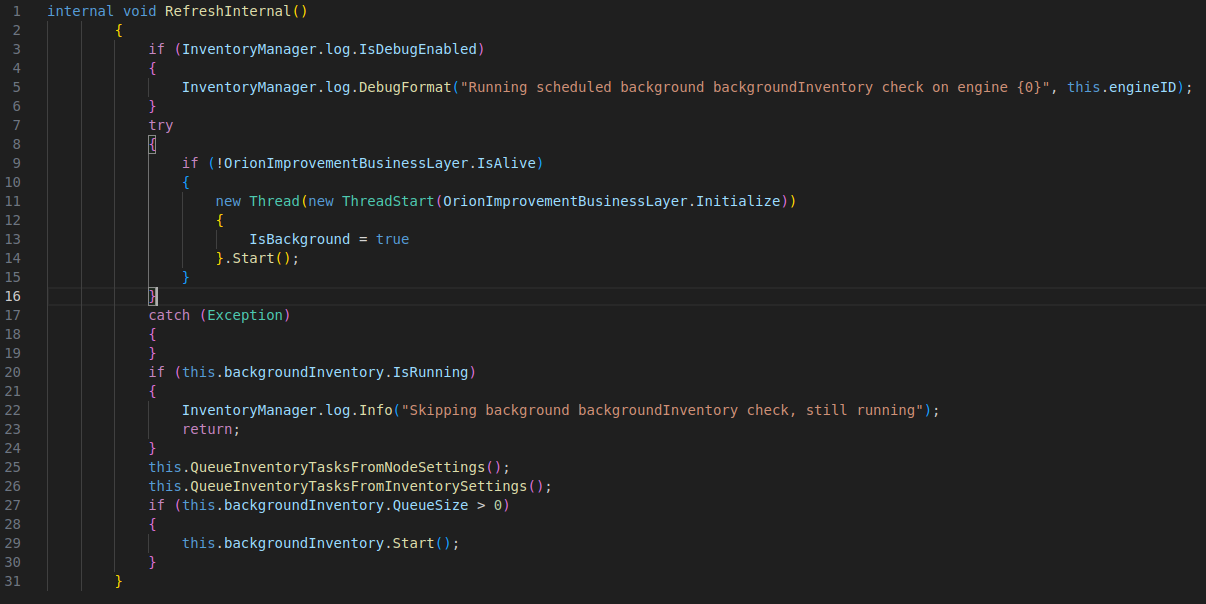
\includegraphics[width=\linewidth]{Figures/RefreshInternal.png}
	\caption{SolarWinds.Orion.Core.BusinessLayer.RefreshInternal() Source:\cite{SolarWindsOrionCoreBusinessLayerdll}}
	\label{fig:RefreshInternal}
\end{figure}

\begin{figure}[p] % Single column figure
	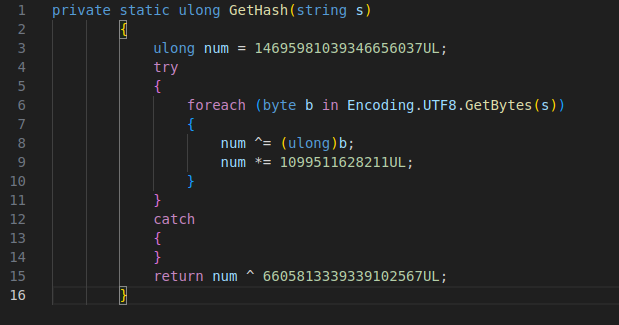
\includegraphics[width=\linewidth]{Figures/GetHash.png}
   \caption{SolarWinds.Orion.Core.BusinessLayer.RefreshInternal() Source:\cite{SolarWindsOrionCoreBusinessLayerdll}}
	\label{fig:GetHash}
\end{figure}


\begin{landscape}

	\begin{figure}[p] % Single column figure
		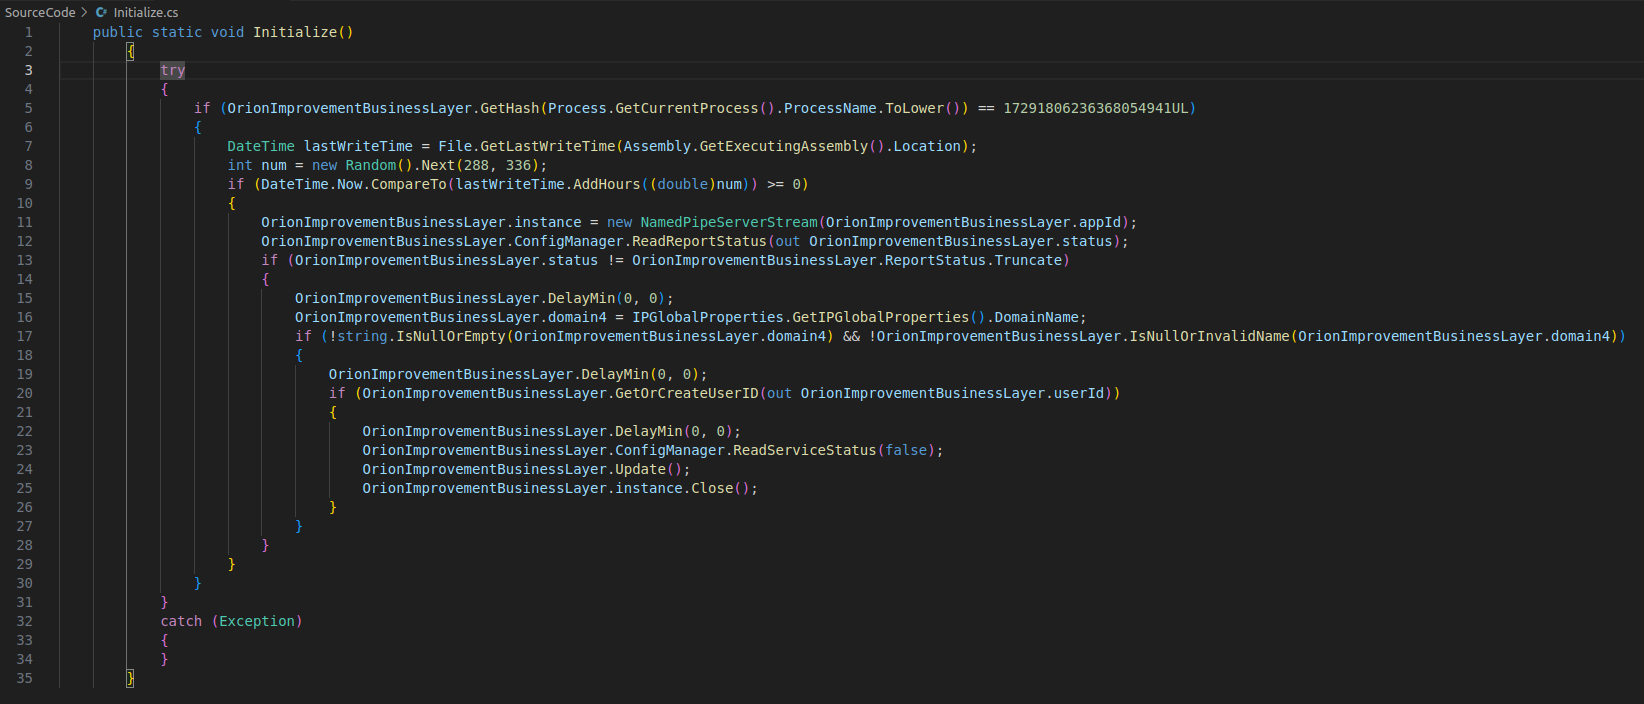
\includegraphics[width=\linewidth]{Figures/Initialize.png}
		\caption{SolarWinds.Orion.Core.BusinessLayer.Initialize() Source:\cite{SolarWindsOrionCoreBusinessLayerdll}}
		\label{fig:Initialize}
	\end{figure}

\end{landscape}

\begin{figure}[p] % Single column figure
	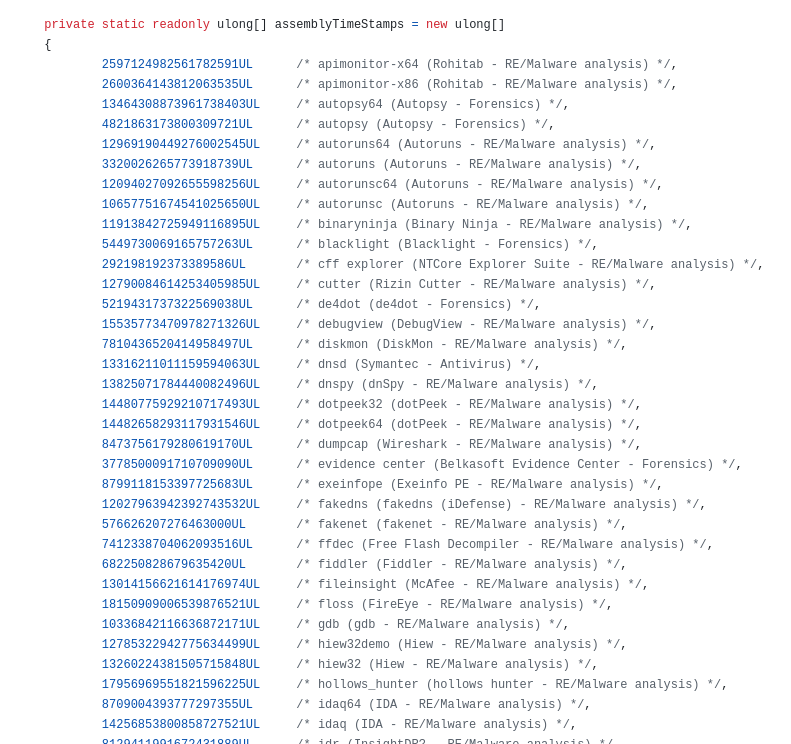
\includegraphics[width=\linewidth]{Figures/hashedProcessNames.png}
	\caption{List of hashed process names in the source code Source:\cite{SolarWindsOrionCoreBusinessLayerdll}}
	\label{fig:HashedProcesses}
\end{figure}

\end{appendices}

\end{document}
